% Chapter Template

\chapter{Sistema d'adaptabilitat} % Main chapter title

\label{DissenySistema} % Change X to a consecutive number; for referencing this chapter elsewhere, use \ref{ChapterX}

Els models UML prèviament descrits ens permeten dissenyar i modelar de forma estandarditzada el sistema de monitoratge. Proporciona, semànticament, tots els recursos necessaris per traduir propostes de configuracions de sistemes en accions reals sobre els monitors implementats.\\

El següent pas és el disseny i implementació d'un sistema que, a partir dels models anteriors, i de tot el domini que defineixen, sigui capaç de gestionar la persistència dels models, obtenir-ne els necessaris per aplicar reconfiguracions, actualitzar els models d'acord a aquestes modificacions, i traduir la informació implícita als models en accions de reconfiguració reals a enviar al sistema de monitoratge.\\

Procedirem a presentar els diferents components que componen aquest sistema.

\section{Model Repository}

El primer component que cal introduir per començar a entendre el \textit{workflow} del sistema d'adaptabilitat és el \textbf{Model Repository}. Aquest component actua en termes genèrics com a un repositori que gestiona la persistència del conjunt de models UML que intervenen en el modelatge del sistema i la seva reconfiguració. Això, per tant, implica tot el conjunt de models descrits anteriorment: \textit{Base Model}, \textit{Feature Model}, \textit{Feature Configuration}, \textit{Pattern Model}, \textit{Profile Model} i \textit{Adaptability Model}.\\

Principalment, les funcionalitats que ha de satisfer són les següents:

\begin{enumerate}
\item Gestionar la persistència dels models en disc
\item Mapejar i encapsular l'estructura de directoris definida per estructurar els models segons el seu tipus
\item Encapsular els mètodes CRUD bàsics per la gestió dels models, aïllant la lògica interna de la resta de components
\item Encapsular mètodes extensius que permetin obtenir models sota unes certes característiques
\end{enumerate}

D'aquesta manera, podem concebre aquest component com una abstracció entre la naturalesa interna dels models i la lògica associada a la càrrega/descàrrega de fitxers amb el nostre sistema, assignant la responsabilitat d'aquests primers punts al Model Repository.\\

Una primera aproximació que ens podríem plantejar seria implementar un component unitari que definís un controlador (que després s'exposaria com a servei per integrar a IF) amb tots els mètodes necessaris per la gestió dels models. Si al nostre sistema únicament resultés d'interès les operacions bàsiques de models, aquesta seria una bona alternativa, ja que estaríem simplificant l'arquitectura del sistema, i hi hauria poc marge per la millora. Però si anem un pas més enllà, i plantegem les necessitats de reconfiguració i adaptabilitat del nostre sistema, veiem que un controlador basat en operacions CRUD únicament ens permetria definir reconfiguracions on tots els models que intervenen en l'adaptació són triats estàticament, no dinàmicament. És a dir: el potencial que oferiria el Model Repository seria referenciar els models implicats en una adaptació mitjançant els seus identificadors, que haurien de ser introduïts manualment.\\

Això per tant implica que no podríem aplicar escenaris d'adaptació com per exemple:\\

\centerline{\textit{Actualitzar el sistema de monitoratge amb la darrera Feature Configuration computada}}\bigskip

Si tornem al cicle \textit{MAPE-k}, suposant un sistema de \textit{\textbf{P}lanificació} que produeix noves propostes de configuració (FC), aquest enviaria periòdicament aquests models al nostre sistema d'adaptabilitat. Si el nostre sistema és capaç de consultar les dates en què aquestes propostes es van afegint, és capaç de computar quina és la darrera afegida. I en definitiva, és capaç de computar, de forma automàtica i sense necessitat de donar-li cap mena d'informació, quins canvis aplicar al sistema de monitoratge.\\

Aquest escenari és clau pel nostre projecte. L'automatització del nostre sistema ve donada precisament gràcies a la persistència dels models UML i a l'actualització d'aquests, responsabilitat d'un altre sistema, a partir dels quals aquest és capaç de llegir, processar i traduir en modificacions reals sobre les activitats de monitoratge. Aquest escenari, però, és només un exemple de possible escenari d'adaptabilitat, basat en un criteri com la data, que serà el que nosaltres farem servir pel desenvolupament del projecte. Però el potencial està en veure que els criteris poden ser diversos, sempre i quan es treballin amb metadades que podem extreure a partir dels models, com és el cas de la data de generació de les propostes de reconfiguració.\\

Addicionalment a aquest problema, alguns models tenen dependències amb altres models UML. El cas més evident, l'\textit{Adaptability Model}, té dependències amb \textit{Feature Configurations}, que alhora tenen dependències amb \textit{Feature Models}, i també amb \textit{Pattern Models} i \textit{Profile Models}. La resolució i gestió d'aquestes dependències pot arribar a ser extremadament complicada si, al carregar un d'aquests models, necessitem computar i resoldre quines són aquestes dependències cada vegada que volem carregar el Model Repository a memòria per executar una adaptació des del component encarregat d'aquest aspecte, l'Adapter, que satisfent el criteri de distribució del nostre sistema pot no tenir accés al mateix repositori en disc que el Model Repository. \\

Partint d'aquestes necessitats, és evident que necessitem estendre els mètodes de lectura de models a mètodes més complerts, on utilitzem dades auxiliars per fer cerques dins el nostre repositori. És en aquest punt quan aquesta primera aproximació resulta ineficient: si volem accedir a les metadades dels fitxers dels models, tals com la data de creació, l'autor, el sistema que l'ha computat, etc. (més endavant les veurem amb més detall), carregar tots els fitxers dinàmicament per accedir a aquestes dades per fer la cerca resulta molt ineficient. És per això que, alternativament, utilitzarem la següent arquitectura per gestionar la persistència de models:

\begin{itemize}
\item \textbf{Model Repository Manager.} Component que gestiona les metadades dels models, emmagatzemades en una base de dades relacionals, i que estén un controlador amb els mètodes de cerca per obtenir les metadades dels models desitjats.
\item \textbf{Model Repository Client.} Component que es comunica amb el Model Repository Manager per obtenir les dades dels models, gestiona la persistència del repositori de models, i encapsula els mètodes i objectes per obtenir i treballar amb els models associats a les reconfiguracions.
\end{itemize}

D'aquesta manera, el primer assumeix les responsabilitats de cerca i gestió de models en base a les seves metadades, i el segon assumeix la responsabilitat principal d'encapsular programàticament l'accés als models, per tal que la resta de components del sistema d'adaptabilitat puguin aïllar-se de la lògica interna d'aquest punt.

\subsection{Model Repository Manager}

Satisfent les necessitats del Model Repository Manager, necessitem contemplar els següents punts:

\begin{enumerate}
\item Disseny i implementació d'una base de dades relacional que emmagatzemi les metadades per cada tipus de model.
\item Disseny i implementació d'un component que accedeixi a la base de dades, i que exposi a través d'un controlador els mètodes de consulta i modificació dels models.
\end{enumerate}

\subsubsection{Disseny de la base de dades}

En primer lloc necessitem definir quines seran les metadades que considerarem per cada model. Generalment, podem considerar que tots els models definits tindran les següents dades:

\begin{itemize}
\item \textbf{Id.} Identificador d'aquell model, únic pel tipus de model (\textit{Base Model}, \textit{Feature Model}...) que representa.
\item \textbf{Name.} Nom del fitxer del model (sense l'extensió).
\item \textbf{AuthorId.} Identificador de l'autor del model.
\item \textbf{CreationDate.} Data de creació del model.
\item \textbf{LastModificationDate.} Data de la darrera modificació del fitxer del model.
\item \textbf{FileExtension.} Extensió del fitxer (.uml, .vql, .yamfc ...)
\item \textbf{SystemId.} Utilitzat dins el context SUPERSEDE per identificar els models que corresponen als diferents escenaris. En el nostre cas, aquest sempre serà \textit{MonitoringReconfiguration}.
\item \textbf{RelativePath.} Ruta relativa del directori \textit{root} on s'emmagatzema el model.
\item \textbf{Dependencies.} Llistat d'identificadors dels models dels quals depèn aquest model.
\end{itemize}

Tot i així, addicionalment existeix la possibilitat d'estendre atributs específics pels diferents models. Considerarem útils pel nostre context els següents:

\begin{itemize}
\item \textbf{Base Model}
\begin{itemize}
\item \textbf{Status.} Indica si el model ha estat computat per un sistema extern (\textit{Computed}), si és el resultat d'una adaptació dins el sistema d'adaptabilitat (\textit{Enacted}), o bé si ha estat dissenyat manualment (\textit{Designed}).
\end{itemize}
\item \textbf{Feature Configuration}
\begin{itemize}
\item \textbf{Status.} Indica si la \textit{Feature Configuration} ha estat computada per un sistema extern (\textit{Computed}), si s'ha aplicat com a adaptació dins el sistema (\textit{Enacted}), o bé si ha estat dissenyada manualment (\textit{Designed}).
\end{itemize}
\item \textbf{Adaptability Model}
\begin{itemize}
\item \textbf{Feature Id.} Identificador de la \textit{feature} referenciada per l'Adaptability Model.
\end{itemize}
\end{itemize}

A partir d'aquestes dades podem procedir al disseny de la base de dades del repositori de metadades. Al existir atributs comuns i atributs diferenciats, hem de decidir quin tipus d'herència apliquem a la base de dades. Recordant les tres opcions, aplicades al nostre cas obtindríem el següent:

\begin{itemize}
\item \textbf{\textit{Single table inheritance.}} Definir una única taula a la base de dades \textit{Model} que inclogui tots els atributs possibles, inclosos els específics, i prengui valors nulls per aquells que no tenen aquell atribut.
\item \textbf{\textit{Class table inheritance.}} Definir una taula genèrica \textit{Model} i N taules addicionals per cada tipus que referenciïn la primera, amb els atributs addicionals per cada cas.
\item \textbf{\textit{Concrete table inheritance.}} Definir una taula per cada tipus de model i replicar els atributs comuns.
\end{itemize}

En el nostre cas, optarem per l'opció \textit{concrete table inheritance}. La raó principal d'aquesta opció és que, tot i compartir la major part de les dades, les entitats de models amb tipus diferents mai tindrà sentit contemplar-les conjuntament. És a dir: qualsevol lectura o modificació de models es farà sobre un model (o conjunt de models) d'un tipus específic, mai sobre models de forma genèrica (no tindrà sentit concebir l'entitat \textit{Model} abstracta). Si considerem la segona opció, veiem que seria molt ineficient, ja que caldria fer \textit{joins} internes per obtenir les dades els models, i per la mateixa raó que la ja esmentada sabem que seria un cost innecessari. Per tant, optarem per definir una taula per cada tipus, mantenint així la independència de les metadades entre models. A l'apèndix ~\ref{AppendixA} podem veure el disseny proposat de la base de dades, d'acord als 6 tipus de models definits.\\

D'aquesta manera, la identificació d'un model queda definida per \textbf{id + ModelType}, el primer com a atribut explícit de metadades i el segon com a metadada implícita derivada de la taula en la qual emmagatzemem el model.

\subsubsection{Disseny i implementació del domini i controlador}

Modelat l'esquema de les metadades a la base de dades, podem procedir a implementar les classes de domini amb les quals treballarem per operar sobre aquestes. Partint del disseny anterior necessitem definir dos aspectes. En primer lloc, necessitem \textbf{modelar la jerarquia} de models, segons els atributs genèrics i els atributs específics de cada model. En segon lloc, definir com modelarem i identificarem el llistat de dependències de cada model.\\

\begin{figure}
\centering
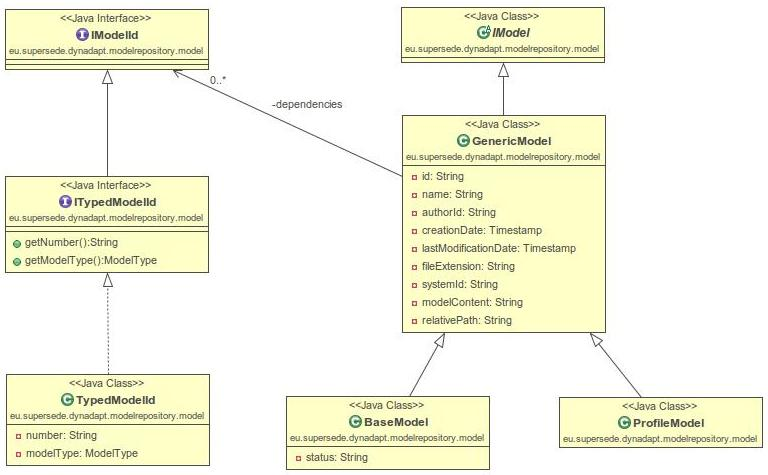
\includegraphics[width=14cm]{Figures/Figure21}
\decoRule
\caption{Disseny del domini del Model Repository Manager}
\label{fig:Figura21}
\end{figure}

A la figura ~\ref{fig:Figura21} es presenta el diagrama simplificat de la proposta de disseny. Per la definició dels models, definim una classe genèrica \textit{GenericModel} amb tots els atributs genèrics a tots els models. Addicionalment, s'implementa una classe per cada tipus de model específic (al diagrama apareixen \textit{BaseModel} i \textit{ProfileModel}, a mode d'exemple). Als atributs que apareixen al diagrama cal afegir els mètodes \textit{getters} i \textit{setters} tradicionals, no afegits per simplificació de l'esquema, així com els constructors. Per sobre de \textit{GenericModel} definim una classe abstracta \textit{IModel}, requisit establert per SUPERSEDE per futures extensions. \\

Paral·lelament es presenta una proposta de gestió de les dependències. Ja que els nostres models es troben identificats per la parella \textit{id + ModelType}, es proposa la definició d'una interfície \textit{IModelId} genèrica, totalment genèrica i sense cap mètode, oberta a possibles extensions i refactoritzacions necessàries pel context de SUPERSEDE. Per gestionar aquestes dependències pel nostre context, definim una nova interfície, \textit{ITypedModelId}, que defineix els mètodes per extreure les dues dades necessàries per identificar un model, \textit{getNumber} i \textit{getModelType}. D'aquesta interfície definim una implementació, que obté aquests dos valors definits als mètodes anteriors mapejant directament aquests atributs. D'aquesta manera, el llistat de dependències dels models usats en la reconfiguració de monitors seran instàncies de la classe \textit{TypedModelId} amb els dos atributs \textit{id} i \textit{ModelType}.\\ 

Amb aquest domini podem procedir a implementar el controlador i, posteriorment, la seva exposició com a servei REST per la integració amb IF. Sense entrar en gaires detalls tècnics sobre aquesta part (molt similar a les anteriors exposicions com serveis), definirem les 5 operacions CRUD bàsiques, sempre considerant per \textit{ModelType}. També serà responsabilitat del Model Repository Manager, associada a cadascuna d'aquestes operacions, la gestió del contingut dels models. Aquesta responsabilitat consistirà bàsicament en emmagatzemar en disc, segons on es trobi desplegat aquest component, els fitxers dels models, amb el contingut determinat. Aquesta persistència es gestionarà definint el contingut del model com un string, tant per indicar al Model Repository Manager el contingut a emmagatzemar, com per obtenir-lo quan es consultin les dades d'un mateix.

\begin{enumerate}
\item \textbf{Llista models d'un tipus.} Retorna les metadades de tots els models existents d'un tipus determinat.
\item \textbf{Obté un model.} Retorna les metadades i un string amb el contingut d'un model donat un identificador i un \textit{ModelType}.
\item \textbf{Crea un nou model.} Emmagatzema un nou model amb les metadades passades al Model Repository Manager i guarda un fitxer a disc amb el contingut, el nom i l'extensió determinats a les metadades.
\item \textbf{Actualitza les metadades d'un model.} Donat un identificador i un \textit{Model Type}, actualitza els valors de les metadades d'un model i el contingut, nom i/o extensió del fitxer (quan s'escaigui). 
\item \textbf{Eliminar les metadades d'un model.} Donat un identificador i un \textit{Model Type}, elimina la instància de metadades d'aquest model i elimina el fitxer del repositori.
\end{enumerate}


\begin{figure}
\centering
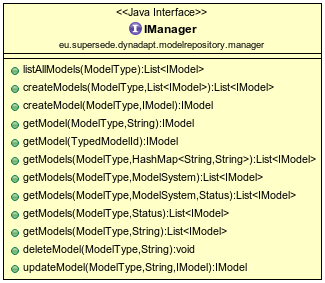
\includegraphics[width=9cm]{Figures/Figure27}
\decoRule
\caption{Disseny de la interfície del Model Repository Manager}
\label{fig:Figura27}
\end{figure}

A l'apèndix ~\ref{AppendixA} es troba definida l'API utilitzada per la integració d'aquest component.

\subsection{Model Repository Client}

Aquest subcomponent del Model Repository s'encarrega d'actuar de pont entre el Model Repository Manager, que gestiona les dades/metadades dels models, i l'Adapter, component que utilitzarà el Model Repository per obtenir les instàncies dels models que necessita per gestionar les adaptacions de reconfiguracions. El disseny i la implementació d'aquest component han estat principalment realitzats per partners tercers del projecte, amb algunes col·laboracions i aportacions específiques per l'adaptabilitat dels models, especialment per la seva orientació a validar el cas d'ús de reconfiguració de monitors. Per tant, procedirem a explicar únicament aquells aspectes realitzats com a part del treball d'aquest TFG i els conceptes necessaris per entendre el seu funcionament.\\

Des d'un punt de vista de \textbf{disseny}, aquest component defineix una interfície \textit{IModelRepository} que defineix, per una banda, els mètodes CRUD per cadascun dels 6 tipus de models existents al sistema. Addicionalment, defineix mètodes de cerca més complexos en base a les metadades dels models. Aquests mètodes seran els que ens permetran executar les adaptacions de forma automatitzada, sense necessitat de definir models específics, a mode de l'exemple introduït anteriorment sobre la cerca de la darrera configuració computada. D'aquests mètodes, ens interessaran especialment els següents:

\begin{figure}
\centering
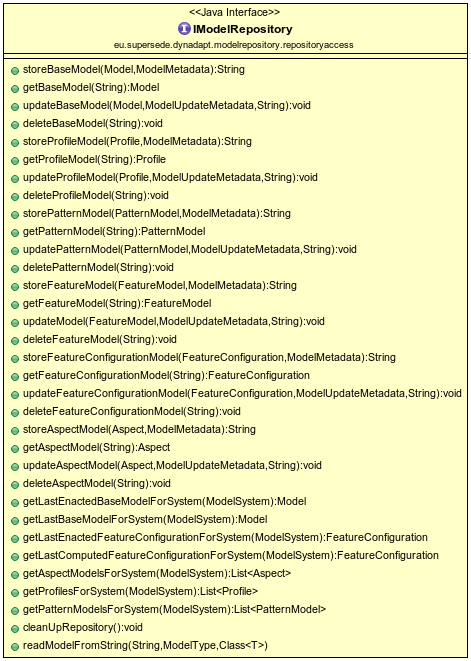
\includegraphics[width=14cm]{Figures/Figure25}
\decoRule
\caption{Disseny de la interfície del Model Repository Service}
\label{fig:Figura25}
\end{figure}

\begin{itemize}
\item \textbf{Obté el \textit{Base Model} més actual} - Permet obtenir el darrer \textit{Base Model} del sistema, que representa per tant l'estat actual del sistema de monitoratge, i ens servirà per agafar com a model per aplicar els canvis de reconfiguració
\item \textbf{Obté la darrera \textit{Feature Configuration} computada} - Obté la darrera \textit{Feature Configuration} amb l'atribut \textit{status} amb valor \textit{Computed}. D'aquesta manera, podem obtenir aquella darrera proposta de configuració que no s'ha executat encara (i per tant, que no té l'atribut \textit{status} amb valor \textit{Enacted})
\item \textbf{Obté la darrera \textit{Feature Configuration} executada} - Obté la darrera \textit{Feature Configuration} amb l'atribut \textit{status} amb valor \textit{Enacted}. D'aquesta manera, podem obtenir la darrera configuració executada, i juntament amb l'anterior mètode, podem computar les diferències entre les dues.
\item \textbf{Obté els \textit{Adaptability Models} candidats} - Obté el llistat de \textit{Adaptability Models} donat un \textit{systemId}. En el nostre cas, ens interessar obtenir aquells amb sistema \textit{MonitoringReconfiguration}, que representaran totes les adaptacions possibles a aplicar dins el nostre context.
\end{itemize}

La implementació d'aquesta interfície defineix la interacció amb el Model Repository Manager i la gestió de persistència dels models per tal de poder referenciar i treballar amb ells des del component Adapter. Podem veure-la definida a la figura ~\ref{fig:Figura25}. Degut a la seva extensió, i per major llegibilitat, fixem-nos que els primers mètodes es tracta dels 4 mètodes CRUD per cada \textit{ModelType} dels quals n'hi ha 6 (i per tant, 24 mètodes amb les operacions bàsiques). A continuació trobem els mètodes anteriorment descrits, que utilitzarem per processar l'adaptabilitat de models i la posterior reconfiguració de monitors.

\section{Model Adapter}

L'adaptació dinàmica de models UML pot arribar a ser complexa, especialment si volem definir una adaptació de models que sigui prou genèrica com per a estendre-la a diferents tipus de models i diferents tipus d'operacions. No serà igual la modificació d'un diagrama de classes (com és el cas d'aquest projecte) que la modificació de, per exemple, un diagrama d'activitats. Per tal de permetre la seva integració a SUPERSEDE, per tant, cal que la lògica d'aquesta adaptabilitat segueixi una estructura prou abstracta que permeti estendre i implementar els diferents casos d'estudi. Per aquesta raó per desenvolupar el Model Adapter, component que assumirà la responsabilitat d'aquesta adaptació dinàmica, treballarem per una banda el disseny genèric del component, i per altra banda la implementació de la lògica necessària pel seu ús al cas de reconfiguració de monitors.\\

\subsection{Disseny genèric}

El primer que necessitem és definir les diferents operacions que el Model Adapter pot suportar. D'acord amb allò ja definit al \textit{Capítol 8. Modelatge de configuracions}, els \textit{Adaptability Models}, que descriuen el comportament d'aquestes adaptacions, suporten 4 tipus d'operacions: 

\begin{enumerate}
\item \textbf{ADD}. Donat un \textit{BaseModel}, afegeix al punt d'injecció \textit{jointpoint} els elements presents a \textit{AdviceModel}.
\item \textbf{DELETE}. Donat un \textit{BaseModel}, elimina del punt d'injecció \textit{jointpoint} els elements presents a \textit{AdviceModel}.
\item \textbf{REPLACE}. Donat un \textit{BaseModel}, substitueix el punt d'injecció \textit{jointpoint} amb els elements presents a \textit{AdviceModel}.
\item \textbf{UPDATE}. Donat un \textit{BaseModel}, actualitza amb el valor definit els elements (atributs, o \textit{slots}) referenciats.
\end{enumerate}

Aquestes operacions estan contemplades des de l'abstracció del tipus de model que volem adaptar. Independentment d'aquest, si analitzem les 4 operacions, veiem que per una banda les 3 primeres presenten un comportament similar: utilitzen la mateixa informació, i la única variació és quin és el tractament intern. La 4a en canvi (la que serà el nostre cas d'estudi) es diferencia tant per les dades que necessita com pel seu comportament intern, ja que es tracta de la modificació de valors d'atributs d'elements del model. Partint d'aquesta idea, per tant, podem discernir entre dos tipus d'operacions: una orientada a l'adaptació complexa de models (ADD, DELETE, REPLACE) i l'altra a l'actualització de valors (UPDATE). A la figura ~\ref{fig:Figura28} podem veure el disseny de dues interfícies: una genèrica \textit{IModelAdapter} que exposa els dos mètodes principals, i una \textit{Composable} que defineix els 3 tipus d'adaptacions compostes segons el tipus d'element UML que estem modificant. Addicionalment, definim una \textit{ComposableFactory} que actuarà com a factoria de les diferents implementacions de \textit{Composable}. Aquest disseny queda justificat pel fet que l'Adapter, el component encarregat d'ordenar al Model Adapter l'adaptació de models, ha d'estar el màxim desacoblat de la lògica específica de l'adaptació de models. Ens veiem forçats a discernir entre UPDATE i la resta degut a la seva diferència des del punt de vista de requisits; però com que no és el cas amb les altres 3 accions, aquestes les encapsulem amb un sol mètode a la interfície \textit{IModelAdapter}, que serà la que aquest Adapter invocarà.\\

\begin{figure}
\centering
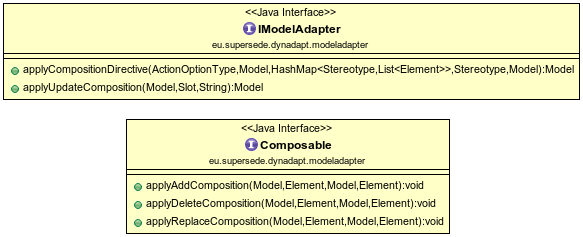
\includegraphics[width=13cm]{Figures/Figure28}
\decoRule
\caption{Disseny de les interfícies del Model Adapter}
\label{fig:Figura28}
\end{figure}

Aquesta interfície \textit{Composable} ens permet exposar els mètodes d'adaptabilitat de models segons cadascun dels 3 tipus d'operacions compostes. En tots casos, els paràmetres rebuts són els mateixos:

\begin{itemize}
\item \textit{Base Model} on s'han d'aplicar els canvis
\item Element etiquetat com a \textit{jointpoint} (o amb el rol corresponent) al \textit{Base Model}
\item \textit{Advice Model} que conté els canvis a aplicar
\item Element etiquetat com a \textit{jointpoint} (o amb el rol corresponent) al \textit{Base Model}
\end{itemize}

Per comprendre millor el disseny i implementació de l'arquitectura genèrica del Model Adapter, la figura ~\ref{fig:Figura30} mostra el diagrama de seqüència de la operació \textit{applyCompositionDirective}, que rep per paràmetre:

\begin{itemize}
\item \textit{actionType} - Instància del tipus d'acció (ADD, DELETE, REPLACE) a executar
\item \textit{baseModel} - Instància del \textit{Base Model} on s'han d'aplicar els canvis
\item \textit{elements} - \textit{Hashmap} identificat per \textit{role} (amb el que s'han etiquetat) amb tots els elements que intervenen en l'adaptació
\item \textit{adviceRole} - \textit{Role} amb el que està etiquetat l'element a l'\textit{Advice Model}
\item \textit{variantModel} - Instància del \textit{Variant Model} que conté els canvis a aplicar
\end{itemize}

\begin{figure}
\centering
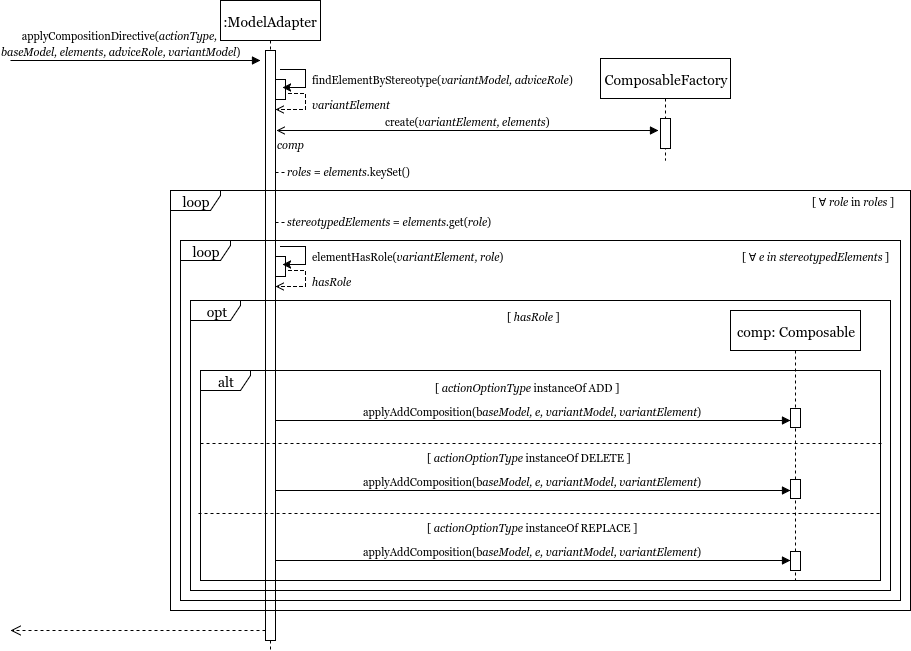
\includegraphics[width=14cm]{Figures/Figure30}
\decoRule
\caption{Diagrama de seqüència de l'adaptació composta del \textit{Model Adapter}}
\label{fig:Figura30}
\end{figure}

\subsection{Implementació - diagrames de classes}

Amb aquest disseny podem estendre els casos d'ús del Model Adapter segons la necessitat d'adaptació de model de cada cas d'estudi del sistema. Al definir amb interfícies les 4 operacions bàsiques, així com els paràmetres d'entrada i la lògica des que rep una petició fins que identifica i ressol la operació a aplicar, només necessitem estendre la implementació per personalitzar les operacions que aplica sobre el model per aplicar les 3 operacions ADD, DELETE i REPLACE.\\

Utilitzant el disseny definit a la figura ~\ref{fig:Figura28},podem estendre la implementació del Model Adapter per tal que treballi amb models UML de tipus diagrama de classes. Amb aquest objectiu, necessitem identificar els dos elements UML bàsics amb els quals treballarem: \textbf{classes} (p.e. la inserció d'un nou monitor) i \textbf{instàncies} (p.e. l'eliminació d'una configuració dins el sistema). Per tant, necessitem dues implementacions de la interfície \textit{Composable}: \textit{ComposableClass} i \textit{ComposableInstanceSpecification}. A la figura ~\ref{fig:Figura31} podem veure el disseny d'aquestes dues implementacions; bàsicament consisteix en la implementació dels 3 mètodes per cada tipus d'operació.\\

\begin{figure}
\centering
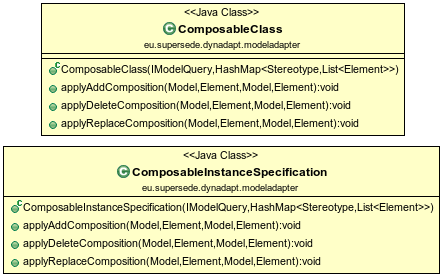
\includegraphics[width=11cm]{Figures/Figure31}
\decoRule
\caption{Implementacions de la interfície \textit{Composable} per \textit{Class} i \textit{InstanceSpecification}}
\label{fig:Figura31}
\end{figure}  

La implementació interna d'aquestes classes s'ha realitzat de forma conjunta amb altres \textit{partners} del projecte, i en qualsevol cas, al no formar part del cas de validació d'aquest TFG, sinó d'una base a partir de la qual plantejar nous escenaris d'extensió i treball futur, no aprofundirem més en els detalls d'aquesta.\\

\section{Components auxiliars}

Per treballar dinàmicament amb models UML utilitzant llibreries i plugins d'Eclipse (com UML2 i Papyrus respectivament), necessitem algunes funcionalitats addicionals a les implementades al Model Adapter. Al tractar-se de components reutilitzats i a implementats al projecte SUPERSEDE per altres col·laboradors del projecte, els presentarem per tal d'entendre el seu objectiu, les seves característiques i com encaixen dins el nostre projecte, però sense comptabilitzar-los com part del desenvolupament del treball. Aquests dos components seran el \textbf{Model Query} i l'\textbf{Enactor}.

\subsection{Model Query}

El \textbf{Model Query} consisteix en un component de gestió de models UML orientat a la cerca d'elements (classes, instàncies, relacions, atributs...) dins d'aquests models. Aquesta cerca s'utilitza combinant UML2, llibreria utilitzada per la càrrega dinàmica de models, amb VQL, utilitzat per definir patrons de cerca dins de models UML.\\

Aquest component ens serà útil a l'hora de buscar al \textit{Base Model} que volem adaptar aquells elements que volem modificar (és a dir, p.e. els \textit{slots} o atributs el valor dels quals hem de modificar-ne el valor). A la figura ~\ref{fig:Figura23} podem veure la definició de la interfície que implementa Model Query, amb un mètode \textit{query(Pattern)} que rep com a paràmetre el \textit{pattern} amb el qual realitzarà la cerca. La nostra tasca serà, per tant, durant el procés d'adaptabilitat, obtenir el \textit{pattern} que ens interessa (que, si recordem, es troba definit a l'\textit{Adaptability Model}) i cridar a una instància d'aquest component inicialitzada amb el \textit{Base Model} corresponent, que ens retornarà com a resultat una \textit{Collection} amb elements UML trobats pel \textit{pattern}. Al tractar-se d'un component ja implementat fora de l'abast del projecte, no entrarem en els detalls tècnics del seu funcionament.

\begin{figure}
\centering
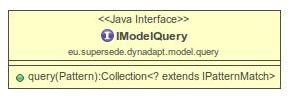
\includegraphics[width=6cm]{Figures/Figure23}
\decoRule
\caption{Disseny de la interfície del Model Query}
\label{fig:Figura23}
\end{figure}

\subsection{Enactor}

El component \textbf{Enactor} és un component orientat a la integració i comunicació entre el sistema d'adaptabilitat i el sistema de monitoratge. La seva tasca principal és rebre com a \textit{input} dos \textit{Base Model}, corresponents a l'actual del sistema abans de la reconfiguració i el nou \textit{Adapted Model} computat de l'adaptació de models, i mitjançant la comparació d'aquests dos models, extreure i construïr peticions de reconfiguració que enviarà posteriorment al component d'entrada del sistema de monitoratge: l'Orchestrator.\\

L'Enactor es tracta d'un component genèric amb característiques pròpies de cada cas d'estudi. Dins el nostre context, l'Enactor ha de ser capaç de computar diferències entre diagrames de classes UML i traduïr-les a reconfiguracions de monitors. Però dins SUPERSEDE aquesta traducció pot ser amb models d'un altre tipus (p.e., diagrames d'activitat) a peticions de reconfiguració d'altres sistemes. Per aquesta raó, es defineixen dos components:

\begin{itemize}
\item \textbf{EnactorFactory.} Classe que encapsula els Enactors de cada \textit{ModelSystem} definit a SUPERSEDE, inclòs \textit{MonitoringReconfiguration}, i que a partir d'aquest paràmetre permet retornar una instància d'Enactor.
\item \textbf{Enactor.} Component encarregat de la traducció de models a peticions de reconfiguració del sistema corresponent. La lògica interna d'aquest dependrà de cada \textit{ModelSystem}.
\end{itemize}

Com en el cas anterior, ignorarem els detalls tècnics interns i ens centrarem únicament en la seva usabilitat. A la figura ~\ref{fig:Figura24} trobem definida la interfície que implementa l'Enactor i la classe EnactorFactory.

\begin{figure}
\centering
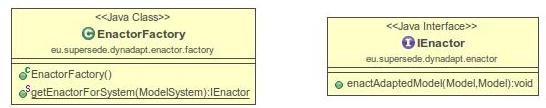
\includegraphics[width=11cm]{Figures/Figure24}
\decoRule
\caption{Disseny de la interfície de l'Enactor i EnactorFactory}
\label{fig:Figura24}
\end{figure}

\section{Adapter}

Satisfets els requisits tècnics i funcionals del Model Repository disposem d'un component que ens permet carregar dinàmicament tots els models i utilitzar els mètodes que la llibreria UML2 defineix amb els mateixos. Paral·lelament, el Model Adapter ens satisfà la necessitat d'adaptació dinàmica de diagrames de classe UML. El següent pas és definir el component que assumirà la responsabilitat de \textbf{gestionar i computar les reconfiguracions}. Aquesta responsabilitat serà assumida per l'Adapter, la responsabilitat principal del qual serà la interacció amb el Model Repository i el Model Adapter per aplicar l'algorisme que a continuació definim per computar reconfiguracions.\\

\subsection{Algorisme d'adaptabilitat}

L'\textbf{algorisme d'adaptabilitat} de models, o bé reconfiguració de monitors pel nostre cas d'estudi, consisteix en la implementació d'un algorisme que resolgui la següent problemàtica:

\begin{center}
\textit{Davant una petició de reconfiguració del sistema, calculem totes les diferències entre la \textbf{darrera Feature Configuration aplicada} i la \textbf{darrera Feature Configuration computada} i trobem totes les diferències de seleccions. Per cada diferència (és a dir, per cada \textbf{selection} present a una de les dues \textbf{Feature Configurations} però no a l'altra), apliquem les \textbf{accions definides als Adaptability Models} corresponents al \textbf{Base Model}, segons si aquesta s'activa a la nova configuració (apareix a la nova FC) o bé es desactiva (no apareix).}
\end{center}

Per entendre millor aquest plantejament, anem a analitzar pas per pas quins són els passos que s'han de realitzar per passar d'identificar una \textit{feature} a modificar el \textit{Base Model}:

\begin{enumerate}
\item Obtenim la \textbf{darrera \textit{Feature Configuration}} amb \textit{status = Computed}, que representa la última configuració del sistema proposada
\item Obtenim la \textbf{darrera \textit{Feature Configuration}} amb \textit{status = Enacted}, que representa la última configuració del sistema aplicada
\item Obtenim el \textbf{darrer \textit{Base Model} del sistema}, que representa l'estat actual del sistema de monitoratge
\item Computem totes les diferències a nivell de \textbf{selections}, que apareixen només a una de les dues \textit{Feature Configurations}.
\item Per cada \textit{selection} diferent trobada:
\begin{enumerate}
\item Obtenim els \textbf{\textit{Adaptability Models} associats a la \textit{feature}} que representa aquella \textit{selection}
\item Per cada \textit{Adaptability Model} obtingut:
\begin{enumerate}
\item Obté tots els \textbf{\textit{pointcuts} definits per l'\textit{Adaptability Model}}
\item Per cada \textit{pointcut} obtingut:
\begin{enumerate}
\item Obté el \textbf{\textit{pattern} definit per aquell \textit{pointcut}}
\item Utilitza el component \textit{Model Query} per trobar tots els \textbf{elements al \textit{Base Model}} segons el \textbf{\textit{pattern} obtingut}
\item Etiqueta amb el \textit{role} definit pel \textit{pointcut} tots els elements trobats pel \textit{Model Query}
\end{enumerate}
\item Obté les \textbf{\textit{compositions} definides per l'\textit{Adaptability Model}}
\item Per cada \textit{composition}:
\begin{enumerate}
\item Comprova si aquella \textit{composition} defineix l'\textbf{activació o desactivació} de la \textit{feature}. 
\item En cas que coincideixi amb el valor de l'activació/desactivació de la \textit{feature}, es comunica amb el Model Adapter per aplicar l'adaptació corresponent i obté el \textit{Base Model} adaptat.
\end{enumerate}
\end{enumerate}
\end{enumerate}
\item Actualitza el Model Repository amb el \textbf{nou \textit{Base Model}} i la \textbf{nova \textit{Feature Configuration}}.
\end{enumerate}

\subsection{Disseny i diagrama de seqüència}

El disseny del component Adapter és relativament senzill en quant a arquitectura software, i el repte important és el disseny i la implementació de l'algorisme prèviament definit. Tot i així, la resta de components del sistema d'adaptabilitat han estat dissenyats i implementats per tal de fer que aquest disseny sigui el més senzill possible.\\

A la figura ~\ref{fig:Figura26} podem veure la interfície definida per l'Adapter. Recordem que, la funció d'aquest component és realitzar l'adaptació de models de forma automàtica mitjançant un únic algorisme genèric. Aquest algorisme és el definit pel mètode \textit{enactAdaptationDecisionActionsForFC(ModelSystem system)}. La resta de mètodes reben paràmetres addicionals ja que estan orientats a realitzar adaptacions no de forma totalment automatitzada, sinó definint paràmetres específics (p.e. definint una nova FC a computar, o bé unes \textit{Actions} específiques). Per exemplificar i validar el nostre projecte, nosaltres ens centrarem en aplicar \textit{Feature Configurations} específiques, per comprovar que els canvis definits satisfan allò especificat a la \textit{Feature Configuration.}\\

\begin{figure}
\centering
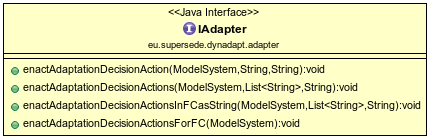
\includegraphics[width=9cm]{Figures/Figure26}
\decoRule
\caption{Disseny de la interfície de l'Adapter}
\label{fig:Figura26}
\end{figure}

A la figura ~\ref{fig:Figura22} podem visualitzar el diagrama de seqüència que defineix l'algorisme prèviament explicat i la seva interacció amb els components que formen part del sistema d'adaptabilitat. 

\begin{figure}[!h]
\centering
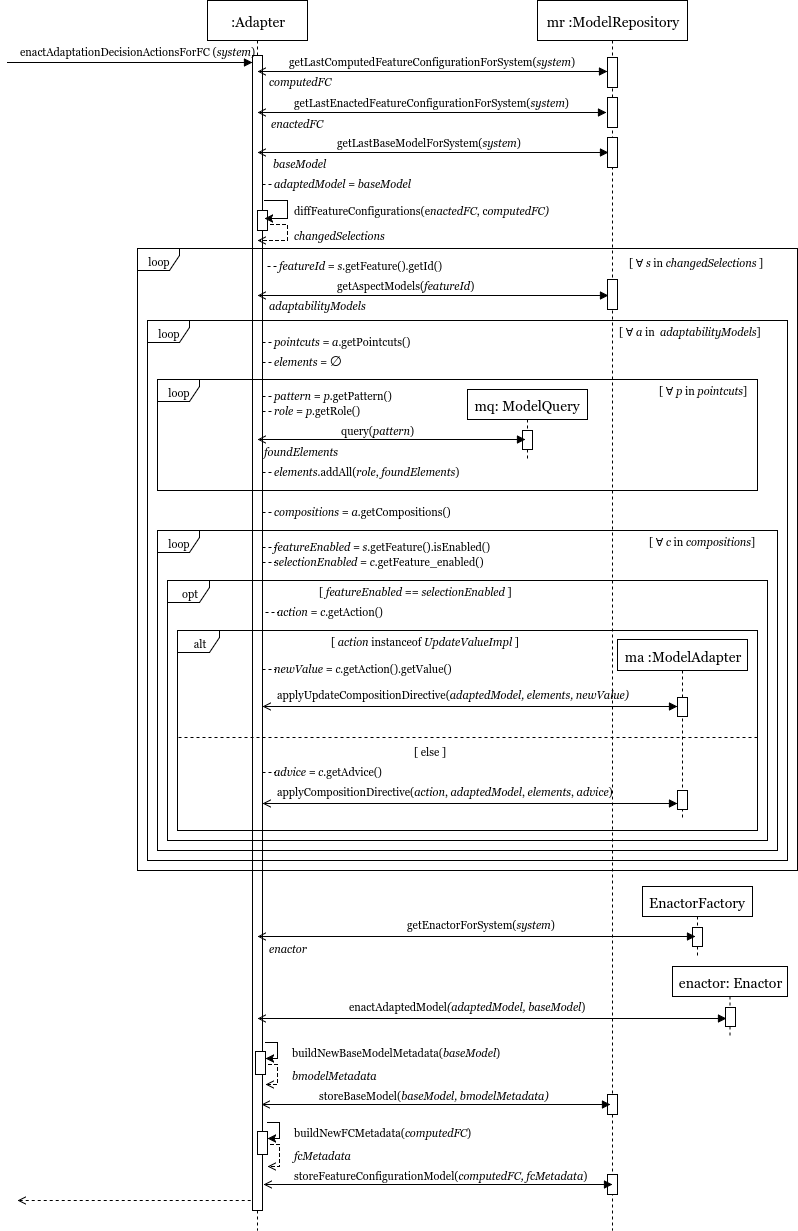
\includegraphics[width=13cm]{Figures/Figure22}
\decoRule
\caption{Diagrama de seqüència de la reconfiguració automàtica del sistema amb l'Adapter}
\label{fig:Figura22}
\end{figure}
